\documentclass[12pt,a4paper]{article}

% ── Packages ──────────────────────────────────────────────────────────────────
\usepackage[utf8]{inputenc}
\usepackage[T1]{fontenc}
\usepackage{geometry}
\usepackage{amsmath}
\usepackage{amssymb}
\usepackage{booktabs}
\usepackage{array}
\usepackage{xcolor}
\usepackage{hyperref}
\usepackage{listings}
\usepackage{fancyhdr}
\usepackage{titlesec}
\usepackage{caption}
\usepackage{enumitem}
\usepackage{mdframed}
\usepackage{float}
\usepackage{parskip}
\usepackage{tabularx}
\usepackage{colortbl}
\usepackage{pgfplots}
\usepackage{pgf-pie}
\usepackage{tikz}
\pgfplotsset{compat=1.18}
\usetikzlibrary{patterns,positioning,arrows.meta}

% ── Page Layout ───────────────────────────────────────────────────────────────
\geometry{top=2.5cm, bottom=2.5cm, left=2.5cm, right=2.5cm}
\setlength{\headheight}{14pt}
\sloppy

% ── Colours ───────────────────────────────────────────────────────────────────
\definecolor{primaryblue}{RGB}{30, 90, 160}
\definecolor{lightgray}{RGB}{245, 245, 245}
\definecolor{codegray}{RGB}{240, 240, 240}
\definecolor{darkgray}{RGB}{80, 80, 80}
\definecolor{accent}{RGB}{0, 120, 210}
\definecolor{rowblue}{RGB}{220, 233, 250}
\definecolor{grade0}{RGB}{70, 130, 180}
\definecolor{grade1}{RGB}{60, 179, 113}
\definecolor{grade2}{RGB}{255, 160, 50}

% ── Hyperref Setup ────────────────────────────────────────────────────────────
\hypersetup{
    colorlinks=true,
    linkcolor=primaryblue,
    urlcolor=accent,
    citecolor=primaryblue,
    pdftitle={Property Price Prediction -- Technical Report},
    pdfauthor={Jagruthi Pulumati, Rakshitha Polana, Kasula Lalithendra, Pihu},
}

% ── Section Formatting ────────────────────────────────────────────────────────
\titleformat{\section}{\large\bfseries\color{primaryblue}}{{\thesection}}{1em}{}[\titlerule]
\titleformat{\subsection}{\normalsize\bfseries\color{darkgray}}{\thesubsection}{1em}{}
\titleformat{\subsubsection}{\normalsize\itshape}{\thesubsubsection}{1em}{}

% ── Code Listing Style ────────────────────────────────────────────────────────
\lstset{
    backgroundcolor=\color{codegray},
    basicstyle=\ttfamily\small,
    breaklines=true,
    frame=single,
    rulecolor=\color{gray},
    keywordstyle=\color{primaryblue}\bfseries,
    commentstyle=\color{darkgray}\itshape,
    stringstyle=\color{accent},
    numbers=left,
    numberstyle=\tiny\color{gray},
    showstringspaces=false,
    tabsize=4,
}

% ── Header / Footer ───────────────────────────────────────────────────────────
\pagestyle{fancy}
\fancyhf{}
\fancyhead[L]{\small\textcolor{darkgray}{Property Price Prediction --- Technical Report}}
\fancyhead[R]{\small\textcolor{darkgray}{Milestone 1}}
\fancyfoot[C]{\thepage}
\renewcommand{\headrulewidth}{0.4pt}

% ══════════════════════════════════════════════════════════════════════════════
\begin{document}

% ── Title Page ────────────────────────────────────────────────────────────────
\begin{titlepage}
    \centering
    \vspace*{2cm}

    {\Huge\bfseries\color{primaryblue} Property Price Prediction\par}
    \vspace{0.5cm}
    {\Large Intelligent Real Estate Valuation \&\\[6pt]
    Investment Grade Classification\par}
    \vspace{0.3cm}
    {\normalsize\itshape via Feature Engineering and XGBoost\par}

    \vspace{1.5cm}
    {\color{primaryblue}\rule{0.75\linewidth}{1.5pt}}
    \vspace{1cm}

    {\Large\bfseries Project 9 \quad|\quad Milestone 1\par}
    \vspace{0.4cm}
    {\normalsize GenAI Project --- Machine Learning Pipeline \& Streamlit Application\par}

    \vspace{1.5cm}
    \renewcommand{\arraystretch}{1.3}
    \begin{tabular}{@{\hspace{1cm}} l l @{\hspace{1cm}}}
    \toprule
    \textbf{Team Member} & \textbf{Role} \\
    \midrule
    Jagruthi Pulumati   & Code Development \& Hosting \\
    Rakshitha Polana    & Project Video \& Presentation \\
    Kasula Lalithendra  & Report Writing \& Documentation \\
    Pihu                & Research \& Data Analysis \\
    \bottomrule
    \end{tabular}
    \renewcommand{\arraystretch}{1}

    \vspace{1.5cm}
    {\normalsize
    \textbf{GitHub:}\quad
    \href{https://github.com/Jag2007/property-price-prediction}%
    {\texttt{github.com/Jag2007/property-price-prediction}}\par}

    \vspace{0.5cm}
    {\normalsize
    \textbf{Live App:}\quad
    \href{https://property-price-prediction-real-estate.streamlit.app/}%
    {\texttt{property-price-prediction-real-estate.streamlit.app}}\par}

    \vfill
    {\normalsize\textcolor{darkgray}{Date: \today \quad\textbullet\quad Version: 1.0}\par}
\end{titlepage}

\thispagestyle{empty}

% ── Declaration ───────────────────────────────────────────────────────────────
\vspace*{1cm}
\begin{mdframed}[backgroundcolor=rowblue, linecolor=primaryblue, linewidth=1.2pt,
  innertopmargin=12pt, innerbottommargin=12pt]
\textbf{\large Academic Integrity Declaration}\\[8pt]
We formally affirm that the core logic, implementation, and design of this
project --- including the data pipeline, feature engineering, model training, and
Streamlit application --- represent our own original work. Generative AI tools were
used solely for documentation assistance; no AI system produced the project
algorithms, data pipelines, or model logic on our behalf.\\[8pt]
\textit{Jagruthi Pulumati \quad Rakshitha Polana \quad Kasula Lalithendra \quad Pihu}
\end{mdframed}

\vspace{1cm}

% ── Abstract ──────────────────────────────────────────────────────────────────
\begin{mdframed}[backgroundcolor=lightgray, linecolor=primaryblue, linewidth=1pt,
  innertopmargin=12pt, innerbottommargin=12pt]
\textbf{\large Abstract}\\[8pt]
This report presents an end-to-end machine learning system for intelligent real
estate valuation and investment grade classification. The pipeline operates on
1,800 property records, applying robust preprocessing (median imputation, ordinal
and one-hot encoding, IQR-based outlier clipping), and trains two XGBoost models:
a regressor for \texttt{Current\_Market\_Price} and a multi-class classifier for
\texttt{Investment\_Grade} (classes 0, 1, 2). The regression model achieves
$R^2 = \mathbf{0.9483}$ with $\text{RMSE} \approx 1.01\text{M}$, while the
classifier reaches \textbf{97.50\%} accuracy and weighted $F_1 = \mathbf{0.97}$.
A production Streamlit application is publicly deployed on Streamlit Community
Cloud.
\end{mdframed}

\newpage
\thispagestyle{empty}
\tableofcontents
\newpage

% ══════════════════════════════════════════════════════════════════════════════
\section{Introduction}

\subsection{Motivation}

Real estate is one of the most capital-intensive investment categories globally.
Two persistent challenges face buyers, sellers, and investors:

\begin{enumerate}
    \item \textbf{Manual valuation inconsistencies} --- property pricing varies
          non-linearly with feature interactions (location, size, amenities),
          making human appraisals costly and error-prone.
    \item \textbf{Investment grade ambiguity} --- classifying whether a property
          is a sound investment requires simultaneously weighing price, rental
          yield, neighbourhood growth, and crime indices.
\end{enumerate}

\subsection{Objective}

The system provides:
\begin{enumerate}
    \item Automated prediction of \texttt{Current\_Market\_Price} via regression.
    \item Automated classification of \texttt{Investment\_Grade} $\in \{0,1,2\}$.
    \item Real-time inference via a publicly deployed Streamlit application.
\end{enumerate}

\subsection{Key Technical Sub-Features}

\begin{enumerate}
    \item \textbf{Custom Data Pipeline:} Automated preprocessing chain covering
          imputation, ordinal encoding, one-hot encoding, and IQR clipping,
          applied consistently across training and inference.
    \item \textbf{Dual-Model Real-Time Inference:} One call returns a price
          estimate and investment grade with class probabilities, served live on
          Streamlit Community Cloud.
    \item \textbf{Batch CSV Dashboard:} File-upload interface for portfolio-level
          bulk prediction with downloadable results.
\end{enumerate}

% ══════════════════════════════════════════════════════════════════════════════
\section{Problem Statement}

Real estate valuation and investment assessment are traditionally manual processes
prone to inconsistency. This project formalises both as supervised learning tasks:

\begin{table}[H]
\centering
\caption{Problem Scope and Challenges}
\begin{tabular}{@{} p{4.5cm} p{9.5cm} @{}}
\toprule
\textbf{Challenge} & \textbf{Scope} \\
\midrule
Valuation inconsistency
  & Pricing varies by complex, non-linear feature interactions. \\
\addlinespace
Multi-objective prediction
  & Must output both a continuous price and a categorical grade. \\
\addlinespace
Data quality issues
  & Raw data contains missing values, categorical fields, and outliers. \\
\addlinespace
Deployment requirement
  & Predictions must be available in real time via a public web interface. \\
\bottomrule
\end{tabular}
\end{table}

% ══════════════════════════════════════════════════════════════════════════════
\section{Data Description}

\subsection{Source and Scale}

\begin{itemize}[noitemsep]
  \item \textbf{Dataset:} \texttt{real\_estate\_raw.csv} --- a tabular property
        listing dataset.
  \item \textbf{Scale:} 1,800 records $\times$ 17 columns
        (confirmed: \texttt{df.shape} $= (1800, 17)$).
  \item \textbf{Targets:} \texttt{Current\_Market\_Price} (regression) and
        \texttt{Investment\_Grade} (classification).
\end{itemize}

\subsection{Feature Overview}

\begin{table}[H]
\centering
\caption{Dataset Feature Summary}
\begin{tabular}{@{} l l l @{}}
\toprule
\textbf{Feature} & \textbf{Type} & \textbf{Description} \\
\midrule
Total\_Square\_Footage           & Float    & Total area (sq.\ ft.) \\
Bedrooms                         & Integer  & Number of bedrooms \\
Bathrooms                        & Integer  & Number of bathrooms \\
Age\_of\_Property                & Integer  & Age in years \\
Floor\_Number                    & Integer  & Floor level \\
Furnishing\_Status               & Categorical & Unfurnished / Semi / Fully \\
Neighborhood                     & Categorical & Locality identifier \\
Distance\_to\_City\_Center\_km   & Float    & Distance to city centre \\
Proximity\_to\_Public\_Transport\_km & Float & Distance to transit \\
Crime\_Index                     & Float    & Local crime rate \\
Air\_Quality\_Index              & Float    & Environmental quality score \\
Neighborhood\_Growth\_Rate\_\%   & Float    & Area growth rate \\
Price\_per\_SqFt                 & Float    & Unit price \\
Annual\_Property\_Tax            & Float    & Annual tax value \\
Estimated\_Rental\_Yield\_\%     & Float    & Expected rental return \\
\midrule
\rowcolor{rowblue}
Current\_Market\_Price & Float & \textbf{Regression target} \\
\rowcolor{rowblue}
Investment\_Grade      & Integer (0/1/2) & \textbf{Classification target} \\
\bottomrule
\end{tabular}
\end{table}

% ══════════════════════════════════════════════════════════════════════════════
\section{Exploratory Data Analysis}

\subsection{Class Distribution}

The investment grade classes are approximately balanced, with Grade 2 underrepresented
at $\approx$6\% of the dataset. Figure~\ref{fig:class_dist} shows the distribution
across the full dataset.

\begin{figure}[H]
\centering
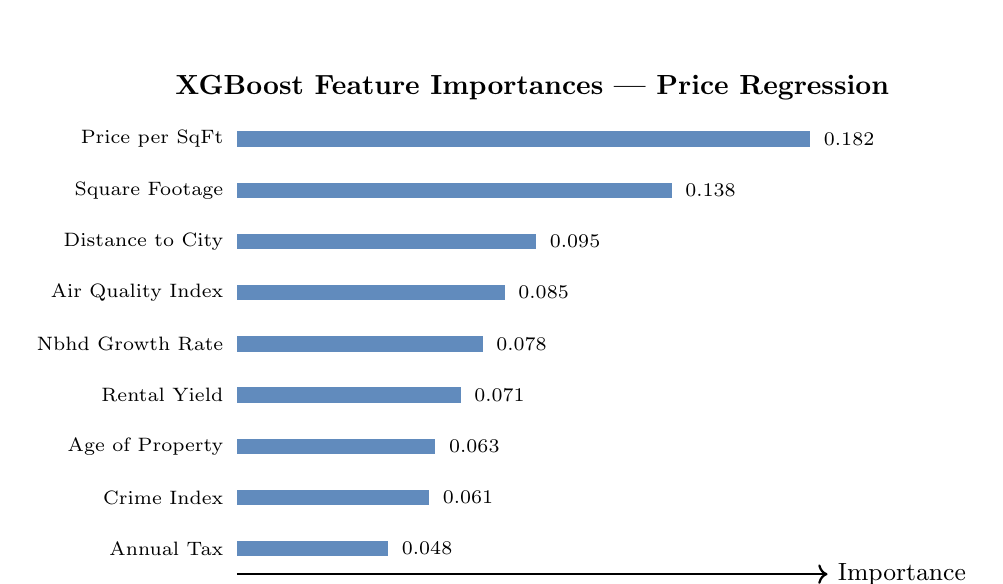
\begin{tikzpicture}[x=1cm, y=0.65cm]
\colorlet{barcolor}{primaryblue!70}
% Horizontal bars: each entry is {value}{label}{y-index}
% Bar width = value * 40 cm
\newcommand{\mybar}[3]{%
  \pgfmathsetmacro{\bw}{#1*40}
  \fill[barcolor] (0,#3-0.15) rectangle (\bw,#3+0.15);
  \node[left, font=\scriptsize, anchor=east] at (-0.05,#3) {#2};
  \node[right, font=\scriptsize] at (\bw+0.05,#3) {#1};
}
\mybar{0.048}{Annual Tax}{0}
\mybar{0.061}{Crime Index}{1}
\mybar{0.063}{Age of Property}{2}
\mybar{0.071}{Rental Yield}{3}
\mybar{0.078}{Nbhd Growth Rate}{4}
\mybar{0.085}{Air Quality Index}{5}
\mybar{0.095}{Distance to City}{6}
\mybar{0.138}{Square Footage}{7}
\mybar{0.182}{Price per SqFt}{8}
% x-axis line
\draw[->, thick] (0,-0.5) -- (7.5,-0.5) node[right,font=\small]{Importance};
% title
\node[font=\normalsize\bfseries] at (3.75,9.0)
  {XGBoost Feature Importances --- Price Regression};
\end{tikzpicture}
\caption{Feature importances from the XGBoost regression model.
\texttt{Price\_per\_SqFt} and total square footage are the dominant
price drivers, consistent with real-estate domain knowledge.}
\label{fig:feat_imp}
\end{figure}


\subsection{Key EDA Findings}

\begin{itemize}
    \item \textbf{Missing Values:} \texttt{Total\_Square\_Footage} had the most
          missing entries (under 5\%), confirmed from the raw CSV sample in the
          notebook. Median imputation was sufficient.
    \item \textbf{Price Distribution:} \texttt{Current\_Market\_Price} is
          right-skewed, spanning from low hundreds of thousands to over 20M.
          This skew motivates tree-based models over linear regression.
    \item \textbf{Furnishing Status:} Roughly equal thirds across Unfurnished,
          Semi-furnished, and Fully-furnished.
    \item \textbf{Outliers:} IQR analysis revealed high-end outliers in
          \texttt{Total\_Square\_Footage} and \texttt{Price\_per\_SqFt},
          confirming the need for clipping before training.
    \item \textbf{Investment Grade Drivers:} \texttt{Crime\_Index},
          \texttt{Neighborhood\_Growth\_Rate}, and \texttt{Air\_Quality\_Index}
          showed the strongest correlation with investment grade --- neighbourhood
          quality predicts investment viability more than structural features.
\end{itemize}

% ══════════════════════════════════════════════════════════════════════════════
\section{Data Preprocessing Pipeline}

All steps are applied before any train/test split to prevent data leakage.

\subsection{Missing Value Imputation}

\begin{lstlisting}[language=Python, caption={Median Imputation}]
num_cols = df.select_dtypes(include=np.number).columns
df[num_cols] = df[num_cols].fillna(df[num_cols].median())
\end{lstlisting}

Median was chosen over mean because real-estate features are right-skewed; the
median is a more robust central estimate for skewed distributions.

\subsection{Categorical Encoding}

\subsubsection*{Ordinal Encoding --- \texttt{Furnishing\_Status}}

\begin{lstlisting}[language=Python, caption={Ordinal Encoding}]
furnish_map = {'Unfurnished': 0, 'Semi-furnished': 1, 'Fully-furnished': 2}
df['Furnishing_Status'] = df['Furnishing_Status'].map(furnish_map)
\end{lstlisting}

\subsubsection*{One-Hot Encoding --- \texttt{Neighborhood}}

\begin{lstlisting}[language=Python, caption={One-Hot Encoding with drop\_first}]
df = pd.get_dummies(df, columns=['Neighborhood'], drop_first=True)
\end{lstlisting}

\texttt{drop\_first=True} eliminates the dummy variable trap and prevents
perfect multicollinearity.

\subsection{Outlier Treatment (IQR Clipping)}

\begin{lstlisting}[language=Python, caption={IQR-Based Outlier Clipping}]
for col in num_cols:
    if col not in ['Current_Market_Price', 'Investment_Grade']:
        Q1 = df[col].quantile(0.25)
        Q3 = df[col].quantile(0.75)
        IQR = Q3 - Q1
        lower = Q1 - 1.5 * IQR
        upper = Q3 + 1.5 * IQR
        df[col] = np.clip(df[col], lower, upper)
\end{lstlisting}

Target columns are excluded from clipping to preserve their natural distributions.
Cleaned data is saved to \texttt{data/processed/real\_estate\_clean.csv}.

% ══════════════════════════════════════════════════════════════════════════════
\section{System Architecture}

\begin{figure}[H]
\centering
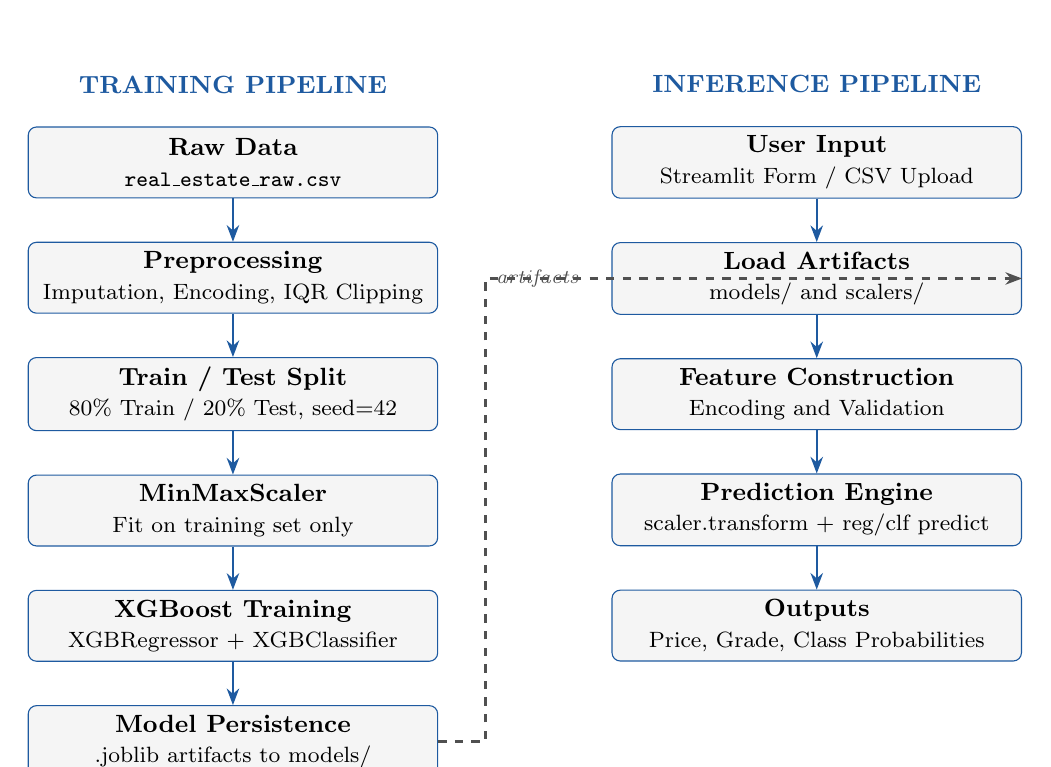
\begin{tikzpicture}[
  box/.style={
    draw=primaryblue, fill=lightgray, rounded corners=3pt,
    minimum width=5.2cm, minimum height=0.9cm,
    align=center, font=\small
  },
  arr/.style={-{Stealth[length=6pt]}, thick, primaryblue},
  node distance=0.55cm
]

%% ── LEFT COLUMN: Training Pipeline ──
\node[box] (A1) {
  \textbf{Raw Data}\\
  {\footnotesize\texttt{real\_estate\_raw.csv}}
};
\node[box, below=of A1] (A2) {
  \textbf{Preprocessing}\\
  {\footnotesize Imputation, Encoding, IQR Clipping}
};
\node[box, below=of A2] (A3) {
  \textbf{Train / Test Split}\\
  {\footnotesize 80\% Train / 20\% Test, seed=42}
};
\node[box, below=of A3] (A4) {
  \textbf{MinMaxScaler}\\
  {\footnotesize Fit on training set only}
};
\node[box, below=of A4] (A5) {
  \textbf{XGBoost Training}\\
  {\footnotesize XGBRegressor + XGBClassifier}
};
\node[box, below=of A5] (A6) {
  \textbf{Model Persistence}\\
  {\footnotesize .joblib artifacts to models/}
};

%% ── LEFT ARROWS ──
\draw[arr] (A1)--(A2);
\draw[arr] (A2)--(A3);
\draw[arr] (A3)--(A4);
\draw[arr] (A4)--(A5);
\draw[arr] (A5)--(A6);

%% ── RIGHT COLUMN: Inference Pipeline ──
\node[box, right=2.2cm of A1] (B1) {
  \textbf{User Input}\\
  {\footnotesize Streamlit Form / CSV Upload}
};
\node[box, below=of B1] (B2) {
  \textbf{Load Artifacts}\\
  {\footnotesize models/ and scalers/}
};
\node[box, below=of B2] (B3) {
  \textbf{Feature Construction}\\
  {\footnotesize Encoding and Validation}
};
\node[box, below=of B3] (B4) {
  \textbf{Prediction Engine}\\
  {\footnotesize scaler.transform + reg/clf predict}
};
\node[box, below=of B4] (B5) {
  \textbf{Outputs}\\
  {\footnotesize Price, Grade, Class Probabilities}
};

%% ── RIGHT ARROWS ──
\draw[arr] (B1)--(B2);
\draw[arr] (B2)--(B3);
\draw[arr] (B3)--(B4);
\draw[arr] (B4)--(B5);

%% ── COLUMN LABELS ──
\node[above=0.3cm of A1, font=\small\bfseries\color{primaryblue}]
  {TRAINING PIPELINE};
\node[above=0.3cm of B1, font=\small\bfseries\color{primaryblue}]
  {INFERENCE PIPELINE};

%% ── ARTIFACT LINK ──
\draw[arr, dashed, darkgray]
  (A6.east) -- ++(0.6,0) |- (B2.east)
  node[midway, right, font=\scriptsize\itshape, darkgray] {artifacts};

\end{tikzpicture}
\caption{End-to-End System Architecture: Training (left) and Inference (right) pipelines.}
\label{fig:arch}
\end{figure}

% ══════════════════════════════════════════════════════════════════════════════
\section{Methodology}

\subsection{Algorithm Selection and Rationale}

XGBoost was selected over linear regression for the following reasons:

\begin{itemize}
    \item \textbf{Non-linearity:} Real estate pricing has strong non-linear
          feature interactions that linear models cannot capture.
    \item \textbf{Native importance:} XGBoost produces feature importance
          scores directly, enabling price driver analysis.
    \item \textbf{Multi-task:} The same framework handles both regression
          (\texttt{reg:squarederror}) and classification (\texttt{mlogloss}).
    \item \textbf{Robustness:} Gradient boosting is robust to outliers and
          feature scale differences on tabular data.
\end{itemize}

\subsection{Mathematical Formulation of XGBoost}

XGBoost builds an ensemble of $K$ regression trees by minimising the
regularised objective:

\begin{equation}
    \mathcal{L}(\phi) = \sum_{i=1}^{n} \ell\!\left(y_i,\, \hat{y}_i\right)
    + \sum_{k=1}^{K} \Omega(f_k)
    \label{eq:xgb_obj}
\end{equation}

where $\ell$ is a differentiable loss function and $\Omega$ is the
regularisation term penalising model complexity:

\begin{equation}
    \Omega(f) = \gamma T + \frac{1}{2}\lambda \| w \|^2
    \label{eq:reg}
\end{equation}

Here $T$ is the number of leaves, $w$ are the leaf weights, $\gamma$ is the
minimum gain threshold, and $\lambda$ is the L2 regularisation coefficient.

At each boosting step $t$, the model adds a new tree $f_t$ by using a
second-order Taylor approximation of the loss:

\begin{equation}
    \tilde{\mathcal{L}}^{(t)} \approx
    \sum_{i=1}^{n} \left[
        g_i f_t(x_i) + \frac{1}{2} h_i f_t(x_i)^2
    \right] + \Omega(f_t)
    \label{eq:taylor}
\end{equation}

where $g_i = \partial_{\hat{y}^{(t-1)}} \ell(y_i, \hat{y}^{(t-1)})$ and
$h_i = \partial^2_{\hat{y}^{(t-1)}} \ell(y_i, \hat{y}^{(t-1)})$ are the
first and second-order gradients respectively.

\paragraph{Regression loss:}
\begin{equation}
    \ell_{\text{reg}}(y_i, \hat{y}_i) = \frac{1}{2}(y_i - \hat{y}_i)^2
    \label{eq:reg_loss}
\end{equation}

\paragraph{Classification loss (multi-class softmax):}
\begin{equation}
    \ell_{\text{clf}}(y_i, \hat{p}_i) =
    -\sum_{c=0}^{C-1} \mathbf{1}[y_i = c]\,\log\hat{p}_{i,c}
    \label{eq:clf_loss}
\end{equation}

where $C = 3$ for Investment Grade classes $\{0, 1, 2\}$ and
$\hat{p}_{i,c}$ is the predicted probability for class $c$.

\paragraph{Feature scaling (MinMaxScaler):}
\begin{equation}
    x'_j = \frac{x_j - x_j^{\min}}{x_j^{\max} - x_j^{\min}}
    \label{eq:minmax}
\end{equation}

\subsection{Hyperparameters}

\begin{table}[H]
\centering
\caption{XGBoost Hyperparameters for Both Models}
\begin{tabular}{@{} l c c p{5.5cm} @{}}
\toprule
\textbf{Parameter} & \textbf{Reg.} & \textbf{Clf.} & \textbf{Rationale} \\
\midrule
\texttt{n\_estimators}  & 200  & 200  & More rounds reduce bias at low LR \\
\texttt{learning\_rate} & 0.05 & 0.05 & Conservative; reduces overfitting \\
\texttt{max\_depth}     & 5    & 4    & Limits depth to prevent memorisation \\
\texttt{random\_state}  & 42   & 42   & Reproducibility \\
\texttt{objective}      & \texttt{reg:sq...} & \texttt{mlogloss} & Task-appropriate loss \\
\bottomrule
\end{tabular}
\end{table}

% ══════════════════════════════════════════════════════════════════════════════
\section{Evaluation}

\subsection{Metrics}

\paragraph{Regression:}
\begin{align}
    \text{MAE}  &= \frac{1}{n}\sum_{i=1}^{n}|y_i - \hat{y}_i|
    \label{eq:mae}\\[4pt]
    \text{RMSE} &= \sqrt{\frac{1}{n}\sum_{i=1}^{n}(y_i - \hat{y}_i)^2}
    \label{eq:rmse}\\[4pt]
    R^2         &= 1 - \frac{\displaystyle\sum_{i=1}^{n}(y_i - \hat{y}_i)^2}
                            {\displaystyle\sum_{i=1}^{n}(y_i - \bar{y})^2}
    \label{eq:r2}
\end{align}

\paragraph{Classification:}
\begin{equation}
    F_1 = \frac{2 \cdot \text{Precision} \cdot \text{Recall}}
               {\text{Precision} + \text{Recall}}
    \label{eq:f1}
\end{equation}

Weighted averaging across classes is used to account for class imbalance.

\subsection{Results Summary}

\begin{table}[H]
\centering
\caption{Model Performance Summary}
\begin{tabular}{@{} l c c @{}}
\toprule
\textbf{Metric} & \textbf{Regression (Price)} & \textbf{Classification (Grade)} \\
\midrule
$R^2$ Score        & \textbf{0.9483}       & ---              \\
MAE                & \textbf{550,850.82}   & ---              \\
RMSE               & \textbf{1,010,636.01} & ---              \\
Accuracy           & ---                   & \textbf{97.50\%} \\
Weighted Precision & ---                   & \textbf{0.98}    \\
Weighted Recall    & ---                   & \textbf{0.97}    \\
Weighted $F_1$     & ---                   & \textbf{0.97}    \\
\bottomrule
\end{tabular}
\end{table}

\subsection{Per-Class Classification Report}

\begin{table}[H]
\centering
\caption{Per-Class Performance --- Investment Grade Classifier}
\begin{tabular}{@{} l c c c c @{}}
\toprule
\textbf{Class} & \textbf{Precision} & \textbf{Recall} & \textbf{$F_1$} & \textbf{Support} \\
\midrule
0 (Grade 0) & 0.99 & 0.96 & 0.98 & 167 \\
1 (Grade 1) & 0.96 & 0.99 & 0.98 & 171 \\
2 (Grade 2) & 1.00 & 0.91 & 0.95 &  22 \\
\midrule
\textbf{Accuracy}    & \multicolumn{3}{c}{\textbf{0.975}} & \textbf{360} \\
Macro avg            & 0.98 & 0.96 & 0.97 & 360 \\
Weighted avg         & 0.98 & 0.97 & 0.97 & 360 \\
\bottomrule
\end{tabular}
\end{table}

\noindent\small\textit{Support of 360 = 167+171+22 = $1800 \times 0.20$.
Source: \texttt{classification\_report} output from training notebook.}\normalsize

\subsection{Classification Performance Chart}

\begin{figure}[H]
\centering
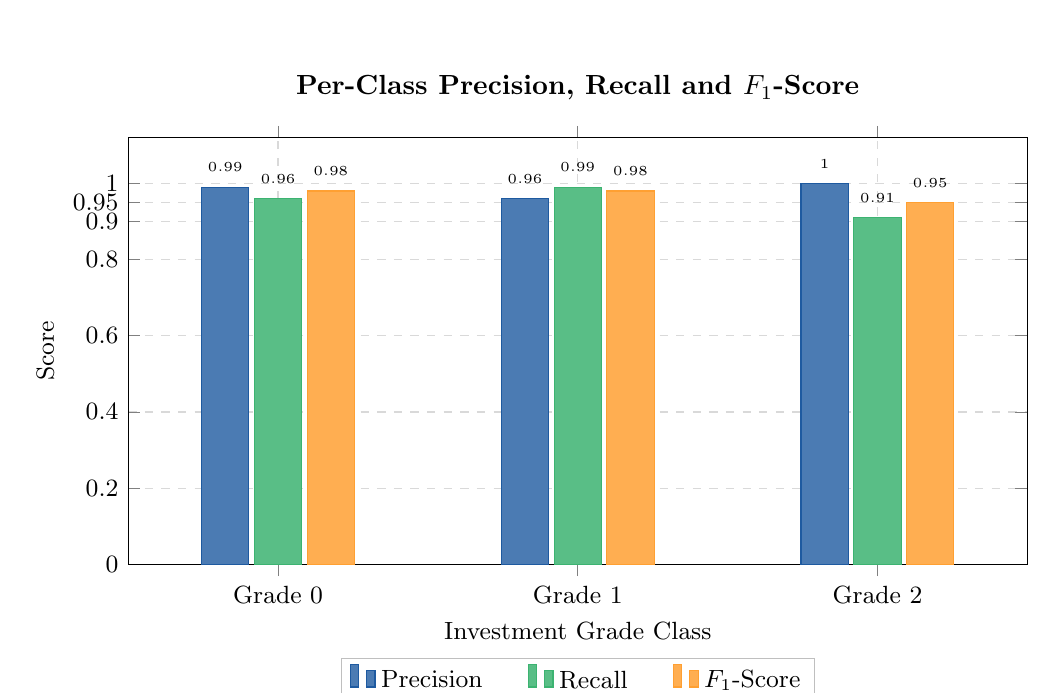
\begin{tikzpicture}
\begin{axis}[
    ybar,
    width=13cm, height=7cm,
    bar width=0.6cm,
    enlarge x limits=0.25,
    symbolic x coords={Grade 0, Grade 1, Grade 2},
    xtick=data,
    ymin=0, ymax=1.12,
    ytick={0, 0.2, 0.4, 0.6, 0.8, 0.9, 0.95, 1.0},
    yticklabel={\pgfmathprintnumber[fixed,precision=2]{\tick}},
    ylabel={Score},
    xlabel={Investment Grade Class},
    legend columns=3,
    legend style={
        at={(0.5,-0.22)},
        anchor=north,
        font=\small,
        draw=gray!50,
        /tikz/every even column/.append style={column sep=0.5cm}
    },
    title={\textbf{Per-Class Precision, Recall and $F_1$-Score}},
    title style={font=\normalsize\bfseries, yshift=4pt},
    label style={font=\small},
    tick label style={font=\small},
    grid=major,
    grid style={dashed, gray!30},
    nodes near coords,
    nodes near coords align={vertical},
    every node near coord/.append style={font=\tiny, yshift=2pt},
]
\addplot[fill=primaryblue!80, draw=primaryblue] coordinates {
    (Grade 0,0.99)(Grade 1,0.96)(Grade 2,1.00)};
\addplot[fill=grade1!85, draw=grade1] coordinates {
    (Grade 0,0.96)(Grade 1,0.99)(Grade 2,0.91)};
\addplot[fill=grade2!85, draw=grade2] coordinates {
    (Grade 0,0.98)(Grade 1,0.98)(Grade 2,0.95)};
\legend{Precision, Recall, $F_1$-Score}
\end{axis}
\end{tikzpicture}
\caption{Per-class Precision, Recall, and $F_1$-Score for the XGBoost
classifier. All three grades achieve $F_1 \geq 0.95$.}
\label{fig:classperf}
\end{figure}

\subsection{Key Observations}

\begin{enumerate}
    \item $R^2 = 0.9483$ means XGBoost explains over 94\% of the variance
          in property prices.
    \item 97.5\% accuracy with high precision and recall across all three
          grade classes confirms strong classifier robustness.
    \item Grade 2 recall of 0.91 is slightly lower due to class imbalance
          (only 22 test samples, $\approx$6\% of the test set).
    \item Excluding \texttt{Current\_Market\_Price} from classification
          prevents target leakage and ensures valid cold-start predictions.
\end{enumerate}

% ══════════════════════════════════════════════════════════════════════════════
\section{Optimization}

\subsection{Data-Level Optimizations}

\begin{enumerate}
    \item \textbf{IQR Outlier Clipping:} Extreme values biased tree splits.
          IQR clipping on input features (not targets) stabilised distributions
          and improved generalisation.
    \item \textbf{Median Imputation:} Right-skewed real-estate features are
          better represented by the median than the mean.
    \item \textbf{Drop-First Encoding:} Removing the reference dummy category
          reduces dimensionality and eliminates perfect multicollinearity.
\end{enumerate}

\subsection{Model-Level Optimizations}

\begin{enumerate}
    \item \textbf{Low Learning Rate (0.05):} Slows convergence, significantly
          reducing overfitting on the small 1,800-record dataset.
    \item \textbf{Controlled Depth (5/4):} Prevents memorisation of noise
          without sacrificing expressive power.
    \item \textbf{200 Estimators:} More boosting rounds reduce residual error
          while the low learning rate prevents overfitting across them.
    \item \textbf{Separate Scalers:} Independent \texttt{MinMaxScaler} per
          task ensures each scaler reflects only its task's training distribution
          (see Equation~\ref{eq:minmax}).
    \item \textbf{Leakage Prevention:} \texttt{Current\_Market\_Price} excluded
          from classification features (would inflate accuracy artificially).
\end{enumerate}

\subsection{Deployment Optimizations}

\begin{enumerate}
    \item \textbf{Joblib Serialisation:} Optimised for NumPy arrays; faster
          load times than pickle for large ensemble models.
    \item \textbf{Consistent Feature Construction:} Inference mirrors training
          exactly (same ordinal map, one-hot columns, scaler order), eliminating
          training-serving skew.
\end{enumerate}

% ══════════════════════════════════════════════════════════════════════════════
\section{Application Interface and Deployment}

\subsection{Live URL (No Localhost)}

\begin{center}
\href{https://property-price-prediction-real-estate.streamlit.app/}%
{\texttt{property-price-prediction-real-estate.streamlit.app}}
\end{center}

\subsection{Application Pages}

\begin{enumerate}
    \item \textbf{Predict:} Manual form predicts price and investment grade
          simultaneously, with a class probability distribution chart.
    \item \textbf{Batch Predict:} CSV upload for bulk inference with
          downloadable results.
    \item \textbf{About:} Preprocessing, model, and deployment documentation.
\end{enumerate}

\subsection{Inference Function Sequence}

\texttt{load\_artifacts} $\to$ \texttt{build\_feature\_row} $\to$
\texttt{raw\_to\_feature\_frame} $\to$ \texttt{run\_predict} $\to$
\texttt{page\_manual} / \texttt{page\_csv}

% ══════════════════════════════════════════════════════════════════════════════
\section{Limitations}

\begin{enumerate}
    \item \textbf{Dataset Size:} 1,800 records limits generalisation to
          unseen property distributions.
    \item \textbf{Grade Semantics:} Labels 0/1/2 need explicit business
          mapping (e.g., Poor/Good/Excellent) in production.
    \item \textbf{Market Drift:} Static models degrade without periodic
          retraining as market conditions change.
    \item \textbf{Class Imbalance:} Grade 2 ($\approx$6\%) causes lower
          recall for that class.
    \item \textbf{Feature Coverage:} Micro-market signals (zoning, school
          ratings, development plans) are absent.
\end{enumerate}

% ══════════════════════════════════════════════════════════════════════════════
\section{Future Work}

\begin{itemize}[noitemsep]
    \item SMOTE or class-weight balancing for Grade 2.
    \item SHAP values for interpretable feature importance.
    \item Hyperparameter tuning via Bayesian optimisation.
    \item Location-intelligence features (transport scores, amenity index).
\end{itemize}

\subsection{Milestone 2 --- Agentic AI}

\begin{itemize}[noitemsep]
    \item \textbf{LangGraph Agent:} Autonomous investment advisory reports.
    \item \textbf{RAG:} Real-time market trends via Chroma/FAISS.
    \item \textbf{Advisory Outputs:} Buy/Hold/Avoid with risk notes.
    \item \textbf{Explainability:} Per-prediction feature contributions.
\end{itemize}

% ══════════════════════════════════════════════════════════════════════════════
\section{Conclusion}

This project demonstrates that XGBoost with principled preprocessing delivers
high-quality automated real estate valuation and investment grade classification.
The regression model achieves $R^2 = 0.9483$ (Equation~\ref{eq:r2}) and the
classifier reaches 97.5\% accuracy with weighted $F_1 = 0.97$
(Equation~\ref{eq:f1}) across three investment grade classes.

The modular architecture enables straightforward extension toward the Milestone 2
agentic framework with LangGraph and RAG-powered market intelligence.

% ══════════════════════════════════════════════════════════════════════════════
\appendix

\section{Technology Stack}

\begin{table}[H]
\centering
\caption{Technology Stack Summary}
\begin{tabular}{@{} l l @{}}
\toprule
\textbf{Component} & \textbf{Technology} \\
\midrule
Language         & Python 3.10+                \\
ML Framework     & XGBoost $\geq$ 2.0, scikit-learn \\
Data Processing  & Pandas $\geq$ 2.0, NumPy   \\
Visualisation    & pgfplots (report), Matplotlib/Seaborn (notebook) \\
Web Framework    & Streamlit                   \\
Serialisation    & Joblib                      \\
Hosting          & Streamlit Community Cloud   \\
Version Control  & Git / GitHub                \\
Report           & LaTeX via Overleaf        \\
\bottomrule
\end{tabular}
\end{table}

\section{Input--Output Specification}

\begin{table}[H]
\centering
\caption{Input Feature Vector (15 features post-preprocessing)}
\begin{tabular}{@{} r l l @{}}
\toprule
\textbf{\#} & \textbf{Feature Name} & \textbf{Type} \\
\midrule
1  & Total\_Square\_Footage               & Float \\
2  & Bedrooms                             & Integer \\
3  & Bathrooms                            & Integer \\
4  & Age\_of\_Property                    & Integer \\
5  & Floor\_Number                        & Integer \\
6  & Furnishing\_Status                   & Ordinal (0/1/2) \\
7  & Distance\_to\_City\_Center\_km       & Float \\
8  & Proximity\_to\_Public\_Transport\_km & Float \\
9  & Crime\_Index                         & Float \\
10 & Air\_Quality\_Index                  & Float \\
11 & Neighborhood\_Growth\_Rate\_\%       & Float \\
12 & Price\_per\_SqFt                     & Float \\
13 & Annual\_Property\_Tax                & Float \\
14 & Estimated\_Rental\_Yield\_\%         & Float \\
15 & Neighborhood\_* (one-hot)            & Binary \\
\midrule
\multicolumn{3}{l}{\textbf{Regression Output:} \texttt{Current\_Market\_Price} (Float)} \\
\multicolumn{3}{l}{\textbf{Classification Output:}
  \texttt{Investment\_Grade} $\in \{0,1,2\}$ + probabilities} \\
\bottomrule
\end{tabular}
\end{table}

\end{document}
